	\section{Nombre: Piso congelado}\label{obs.pisoC}
	\subsection{Descripción}
	Pedazo de hielo congelado en el piso de un terreno, es rígido. Al contacto con el jugador quita toda fricción del piso, ocasionando que no exista suficiente control del jugador de su velocidad y dirección horizontal.
	\subsection{Esquema}
	Ver figura \ref{fig:pisoC}.
	\begin{figure}
		\centering
		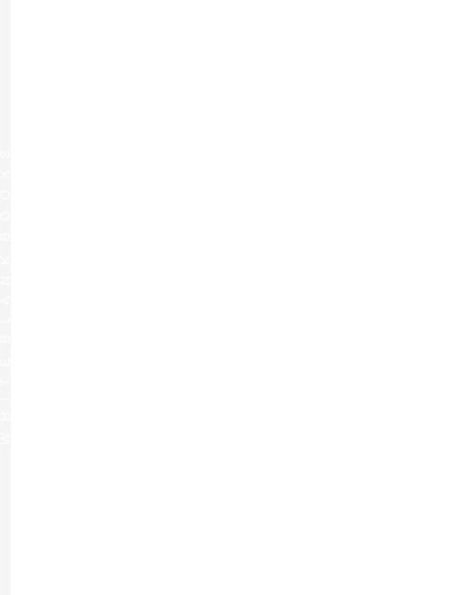
\includegraphics[height=0.2 \textheight]{Imagenes/pisoC}
		\caption{Piso congelado.}
		\label{fig:pisoC}
	\end{figure}